\documentclass[sigconf,letterpaper,10pt,nonacm]{acmart}

% ACM recommends these packages which are already included in acmart
% No need for manual inclusion of graphicx, hyperref, etc.
% Only add packages that aren't already part of acmart

\settopmatter{printacmref=false} % Removes the ACM reference block
\setcopyright{none} % For non-ACM submission
\usepackage{tabularx}
\usepackage{array}
\usepackage{makecell}
\usepackage{booktabs}  % For professional-looking tables
\usepackage{multirow}  % For merged rows in tables
\usepackage{graphicx}  % Already loaded by acmart, but included for completeness
\usepackage{xcolor}    % For colored text
\usepackage{xspace}
\usepackage{caption}
\captionsetup[table]{labelfont=normalfont, textfont=normalfont}
\captionsetup[figure]{labelfont=normalfont, textfont=normalfont}
\usepackage{hyperref}
\usepackage{tcolorbox} % For boxed text
\usepackage{courier}
% Special commands
\newcommand{\todo}[1]{{\color{red} TODO:  {#1}}}
\newcommand{\future}[1]{{\color{blue}{#1}}}
\newcommand{\TK}{{\color{red} TK }}
\newcommand{\nextversion}[1]{{\color{pink}{#1}}}
\begin{document}

\title{Elephant Herd Tracking IoT Application: Design Decisions and Tradeoff Analysis}
\author{Samvrit Srinath}
\email{sasrinath@ucsd.edu}
\affiliation{
  \institution{University of California, San Diego}
  \city{La Jolla}
  \state{California}
  \country{USA}
}

\begin{abstract}
    This report presents the design considerations, energy modeling, structural components, and implementation feasibility of an IoT-based elephant herd tracking application. The system aims to monitor elephant migration patterns in Southern India (where the author is originally from), using a network of infrared-equipped sensor nodes. Inspired by other short range sensors like the ones used in Ring doorbells, the nodes will detect and localize elephants based on heat signatures. The report then concludes the two best wireless technologies for this application, NB-IoT and LoRa, based on a tradeoff analysis of power consumption, data throughput, and cost efficiency. The final design is both cost-effective and energy-efficient, promising a robust solution for real-world wildlife monitoring.
\end{abstract}

\maketitle

%%%%%%%%%%%%%%%%%%%%%%%%%%%%%%%%%%%%%%%%%%%%%%
\section{Introduction \& Application Motivation}
I am originally from Southern India, (in particular a city called Chennai), but when I go to visit my relatives who live in more remote parts of South India, I often hear stories about elephants wandering into villages and causing damage. I am also an Elephant enthusiast and have always been fascinated by these Elephants. This project is a way for me to combine my passion for elephants with real-world design considerations. 

\subsection{Background}
Elephants are a keystone species in the Indian subcontinent, playing a crucial role in forest ecosystems. However, human-elephant conflicts are a significant issue in regions where human settlements overlap with elephant habitats. Monitoring elephant migration patterns is essential for wildlife conservation and to mitigate human-elephant conflicts, as well as to preserve the Quality of Life for both humans and elephants. I localize my study to strictly Southern India to serve as a \textit{pilot} for a larger scale project that could be implemented in other parts of India and the world.

Figure \ref{fig:elephantmap} shows the current elephant migration patterns, especially concentrated in South India, which bolster the need for a system to monitor these elephants. The \textit{Annamadi}, \textit{Nilgiri}, and \textit{Periyar} while located in remote areas, are proximal to many important cities like \textbf{Bangalore}, \textbf{Coimbatore}, and \textbf{Madurai}, aggregating to a total population of over 20 million people\cite{elephantmap}. The need for a system to monitor these elephants is evident, and the system must be low-cost, low-power, and scalable to cover a large area.

\begin{figure}
    \centering
    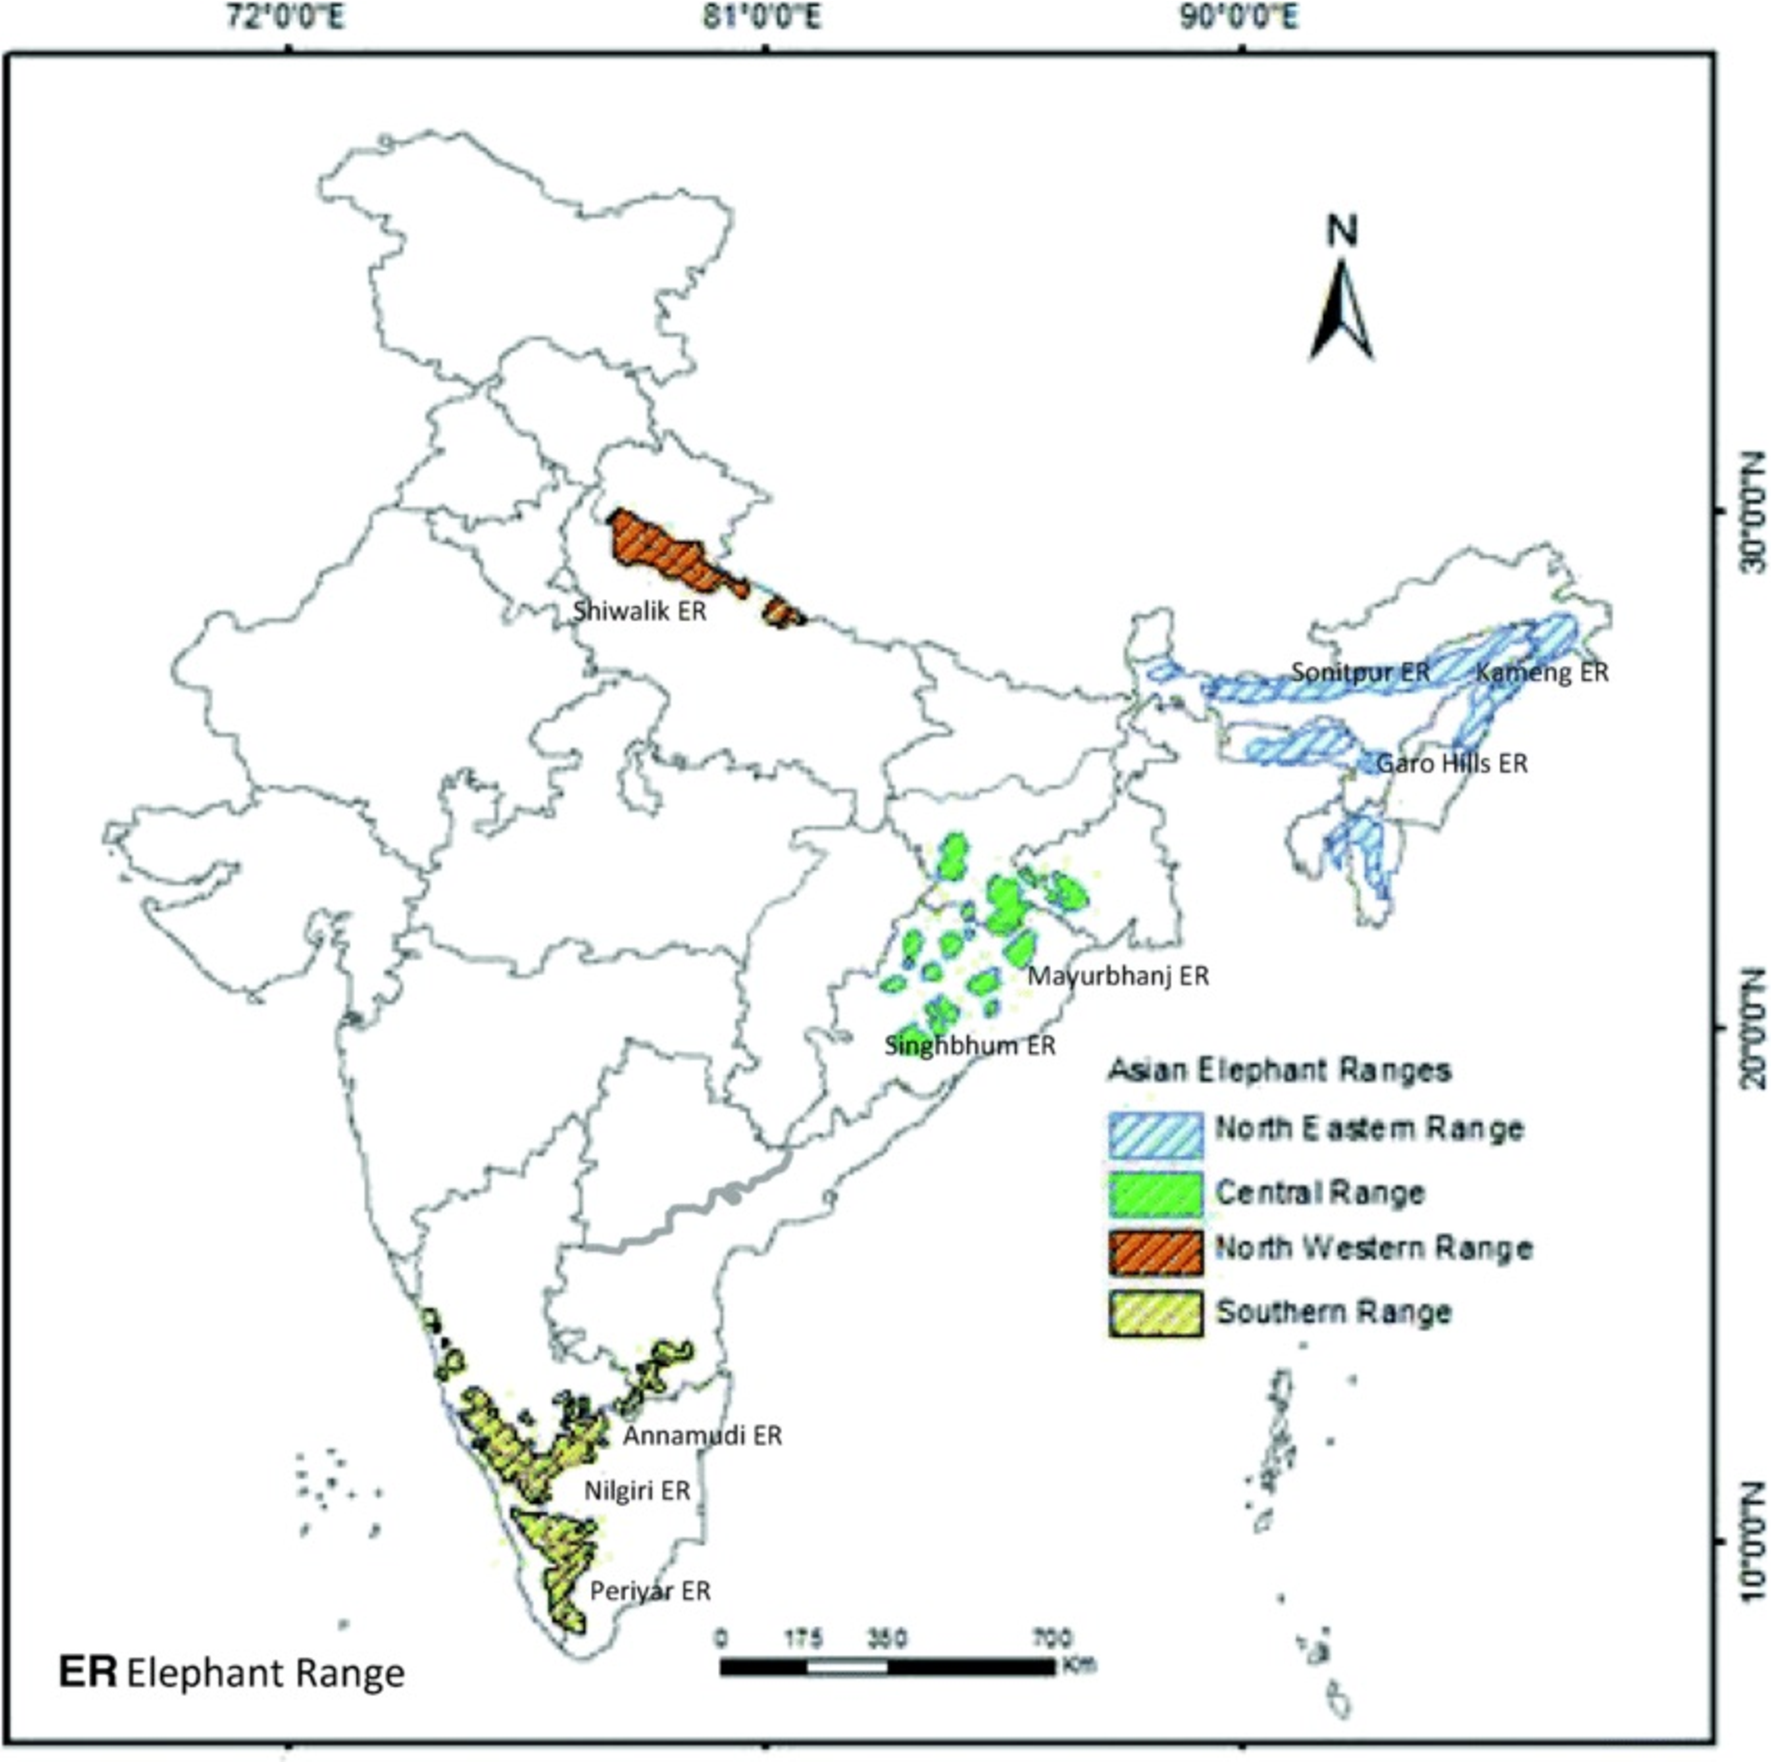
\includegraphics[width=0.9\columnwidth]{figures/Elephant-ranging-areas-in-India.pdf}
    \caption{Map of Current Elephant Migration Patterns and concentrated Habitats in India. Notice the concentration of elephants in the \textit{Annamadi}, \textit{Nilgiri}, and \textit{Periyar} Regions.}
    \label{fig:elephantmap}
\end{figure}

Also another important design consideration is the fact that the elephants habitat are spread in a variety of terrains, usually in high elevation, dense forests, and remote areas. This provides some road blocks in terms of connectivity and power, and also makes it difficult for large scale infrastructure to be built (i.e. cell phone towers, power lines, etc.). So relative to each sensor node, the system must be self-sufficient in terms of power for our pilot study, and must be able to communicate over long distances.

\begin{figure}
    \centering
    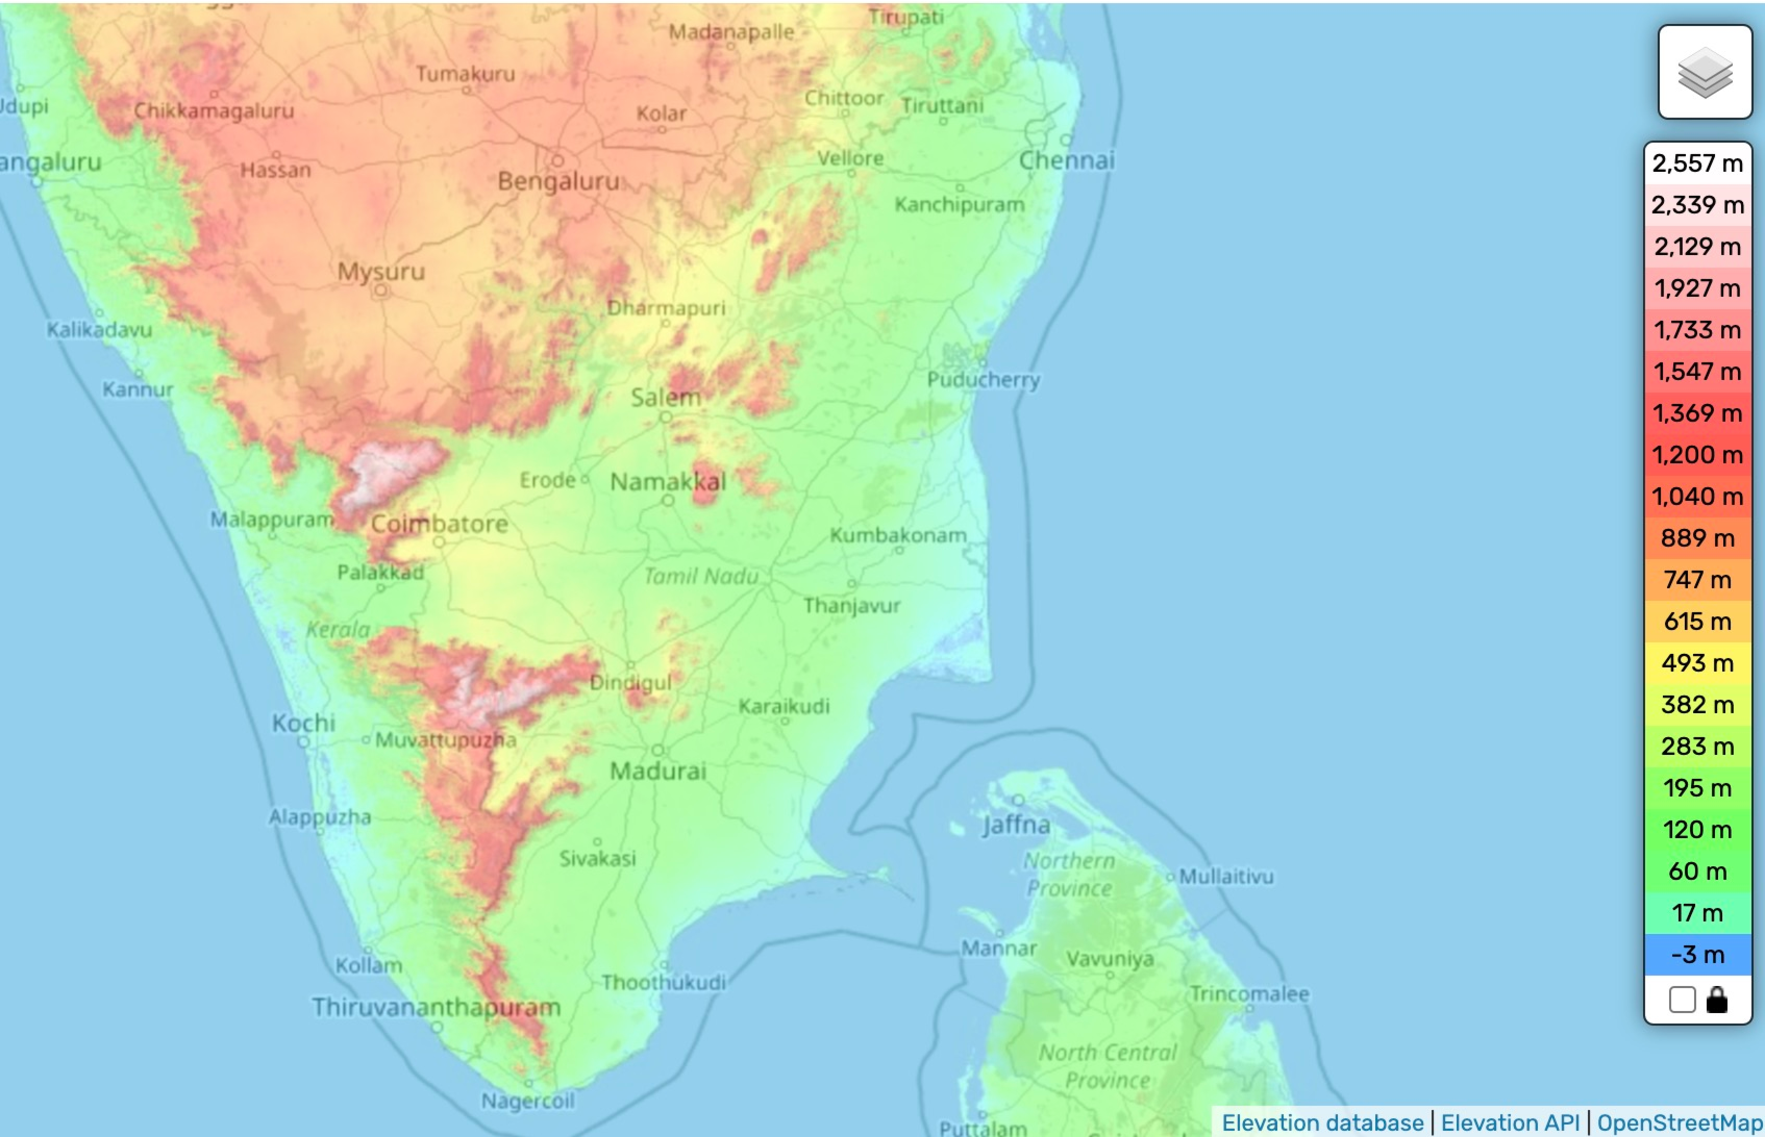
\includegraphics[width=0.9\columnwidth]{figures/GroundTopology.pdf}
    \caption{Ground Topology of the Elephant Habitat Area.}
    \label{fig:groundtopology}
\end{figure}
\section{Part A: Defining the Application}
\subsection{High-Level Description}
Our goal is to implement a large-scale Elephant Tracking and Monitoring System across the \textbf{Neyyar Wildlife Sanctuary}. This Sanctuary is near cities like \textit{Trivandrum} and \textit{Madurai} and is encircled by many villages. For both the safety of elephants and of residents nearby to this sanctuary, it is crucial to montior the movements of these elephants. The system will consist of a set of \textbf{infrared-equipped} IoT nodes that will detect and beacon out their location based on heat signatures. Infrared will work exceptionally well as it is a \textbf{non-intrusive}, \textbf{non-visible} way to detect elephants. Subsequently, elephants also emit a lot of heat (as an innate property of body heat generated $\propto$ body mass), making it an ideal way to detect elephants.

The size of our deployment will be over several hundred square miles, making range and power efficiency imperative, coupled with the rough and forrested terrain of the sanctuary. 
\begin{figure}[h!]
    \centering
    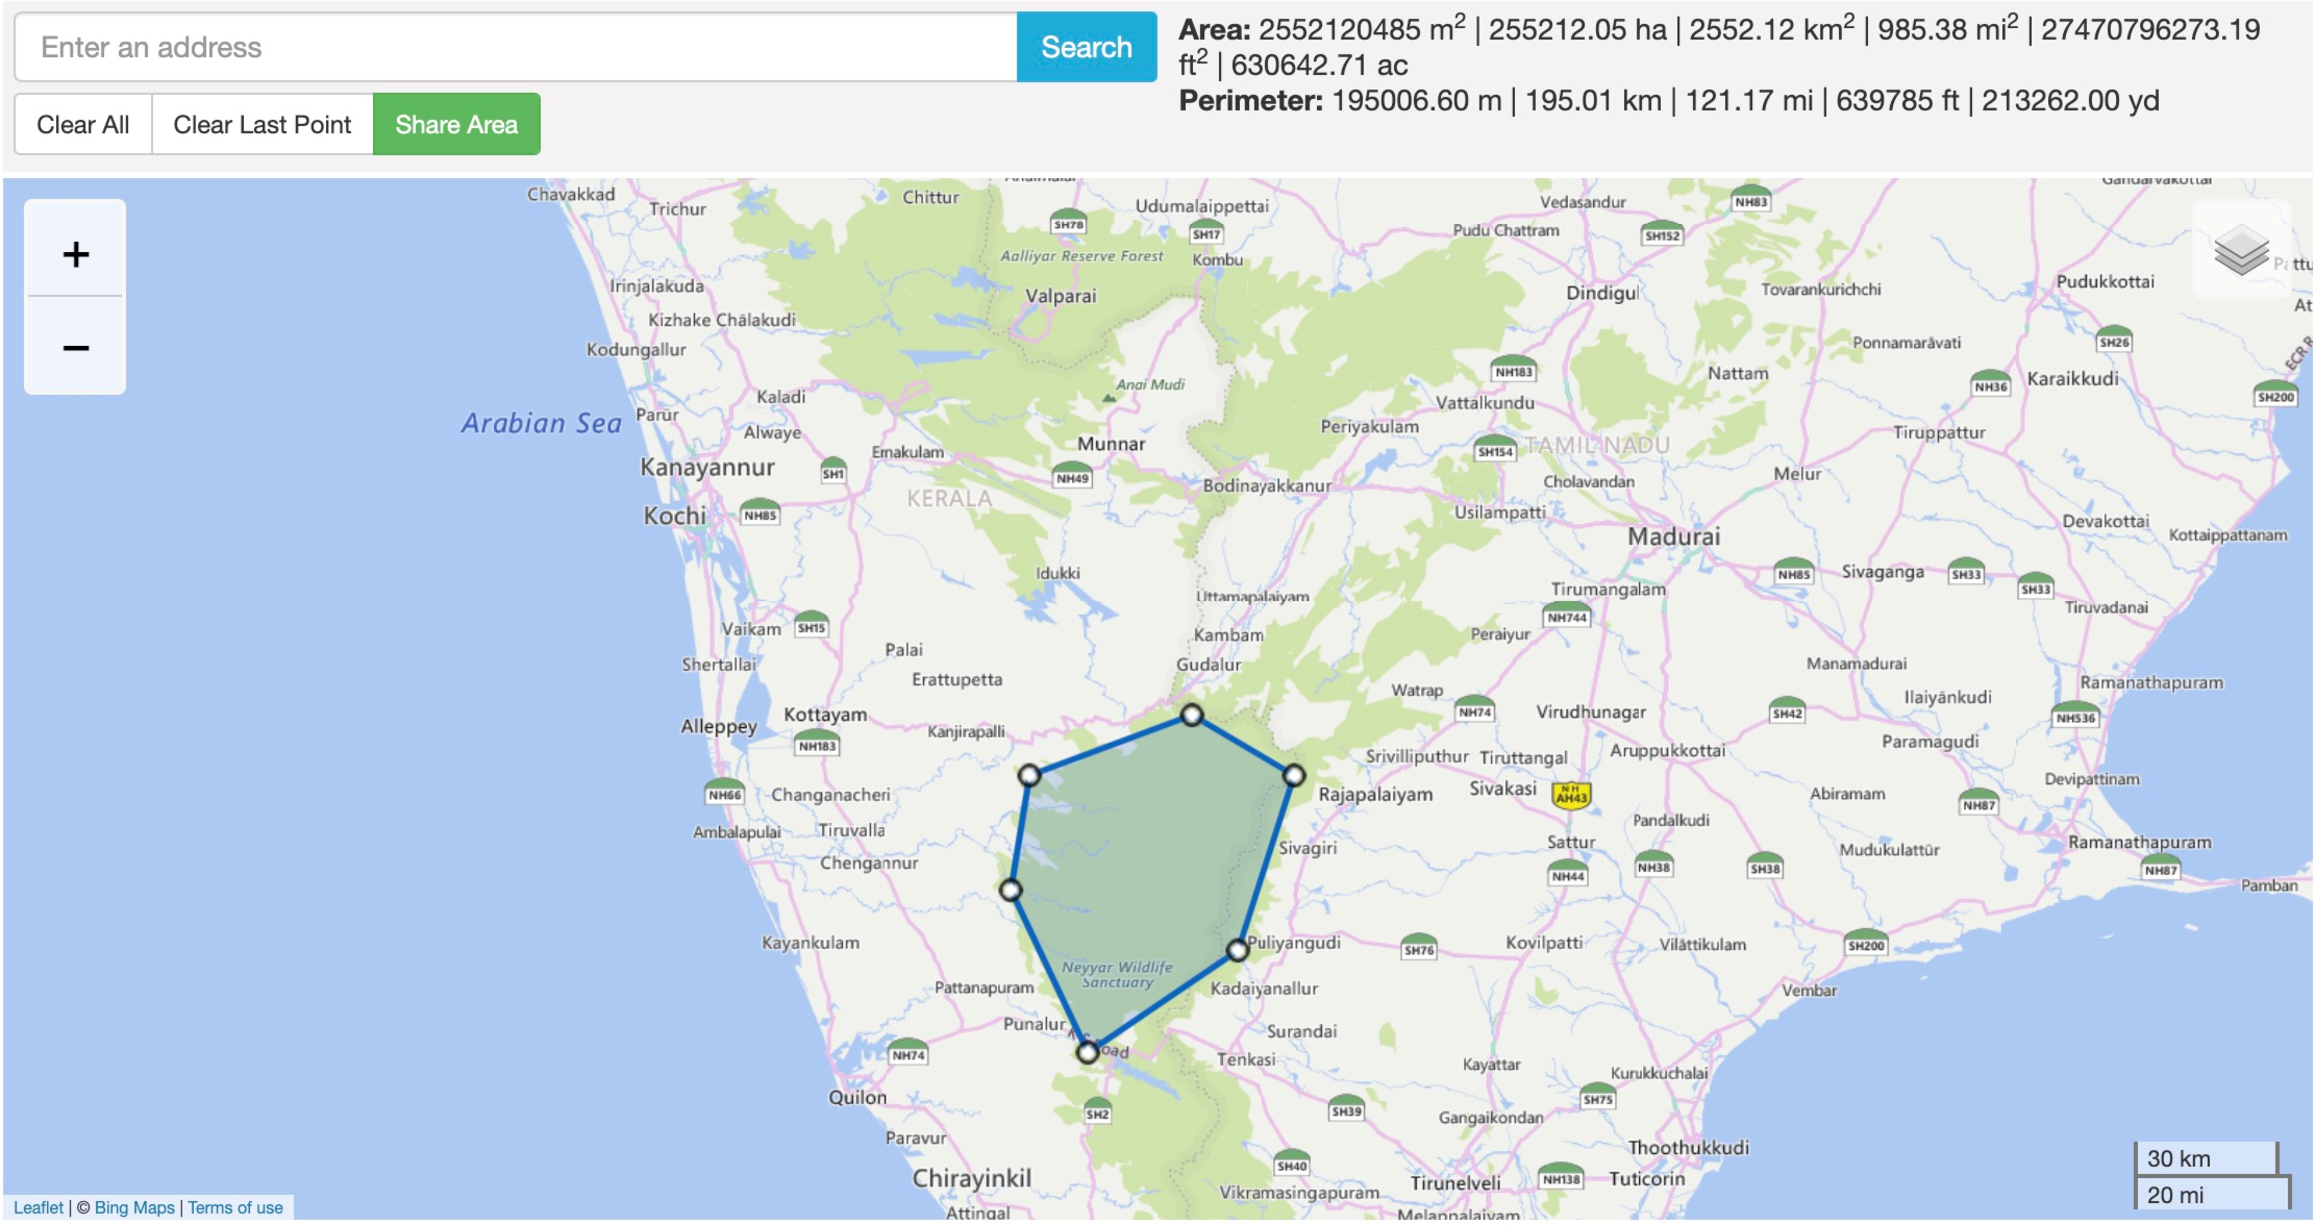
\includegraphics[width=\columnwidth]{figures/NeyyarArea.pdf}
    \caption{Neyyar Wildlife Sanctuary, Kerala, India. Total Area $\approx$ 985 mi$^2$.}
    \label{fig:neyyar}
\end{figure}
There will be three main operating modes for the system: 
\begin{enumerate}
    \item \textit{Steady-State Sensing:} Periodic detection and transmission of location data.
    \item \textit{Event-Driven Update:} Firmware updates and diagnostic data (e.g., when abnormal behavior is detected).
    \item \textit{Emergency Mode:} In the event of an emergency, the system will switch to a high-power mode to ensure that the elephants are tracked and monitored. (i.e. always transmitting location data, sensing etc.)
\end{enumerate}

The role of each of these is similar to what we have seen in our practical applications of IoT devices in Labs. Steady-State Sensing is akin to the Sleepy End Devices that we developed in Lab 3, where we periodically check in with the network and are awoken from sleep should our sensor detect anything or we need to listen from an update from the wider network. Event-Driven Update is akin to the firmware updates that we saw were a necessary condition in Homework 2. Finally, Emergency Mode is just the device will remain on and always transmitting data, in dire situations where an Elephant Habitat is moving towards a village, traffic, or other dangerous areas.

\subsubsection{Steady State Sensing}
In this mode, the nodes will be in a low-power state, waking up periodically to check for elephants. Every 5 minutes, the nodes will simply periodically transmit their location data to a base station. 

Our packet will look like: 
\begin{itemize}
    \item \textbf{Header:} 1 byte
    \item \textbf{Location Data(Latitude, Longitude):} 8 bytes
    \item \textbf{Timestamp:} 4 bytes
    \item \textbf{Elephant Detected/Present}: 1 byte
    \item \textbf{Battery Level:} 1 byte
    \item \textbf{Health Status:} 1 byte
    \item \textbf{Total:} 16 bytes
\end{itemize}

\subsubsection{Event-Driven Update}
In this mode, the nodes will be doing diagnostic work, similar to the firmware updates we saw in Homework 2. Either by clearing out old data, or by checking for any abnormalities in the data that is being collected. Also firmware updates that will be carried out once every month will be done in this mode. (As our application is in a remote area, we cannot afford to have a lot of downtime for the system, so we will have to do firmware updates in a way that does not disrupt the system too much). \textbf{Assumption: } I'll assume that our firmware update will be of a similar scope to the ones we did in Homework 2, so a 10 MB update once a month will be done. 

This means that we do this diagnostic clearing and firmware update once a month, batched, and the other times we are either in Steady State Sensing or Emergency Mode.

\subsubsection{Emergency Mode}
In this mode, the nodes will be in a high-power state, always transmitting data to the base station. This will be done in the event of an emergency, where the elephants are moving towards a village, or a dangerous area. This will be done to ensure that the elephants are tracked and monitored at all times. This means that our sensor is always on, and always transmitting data (i.e we'll set a buffer of 10 seconds, and transmit data every 10 seconds). Rather than doing a periodic check and sleeping, this is more of an \textit{active tracking mode}, where our Infrared Sensor is constantly "pinging the environment", and sending updates on movement of the elephants that are in immediate visibility.

In this mode, the packet structure remains the same to ease the transition between modes, and standardize the data parsing and data transmission efforts. However, the frequency of transmission is increased to every 10 seconds, and the data is always being transmitted. 
\begin{itemize}
    \item \textbf{Header:} 1 byte
    \item \textbf{Location Data(Latitude, Longitude):} 8 bytes
    \item \textbf{Timestamp:} 4 bytes
    \item \textbf{Elephant Detected/Present}: 1 byte
    \item \textbf{Battery Level:} 1 byte
    \item \textbf{Health Status:} 1 byte
    \item \textbf{Total:} 16 bytes
\end{itemize}

\subsection{Data Workload}

Simple dimensional analysis reveals the following data workload for our system. We use the formula
\begin{align*}
    \text{Data Workload} &= \frac{\text{Packet Size}}{\text{Time Interval (s)}} \times \frac{60 \text{ s}}{1 \text{ min}} \\
        &\qquad \times \frac{60 \text{ min}}{1 \text{ hr}} \times \frac{24 \text{ hr}}{1 \text{ day}} \\
        &\qquad \times \frac{30 \text{ days}}{1 \text{ month}}
    \end{align*}
With either $\text{Data Rate} = \frac{16 \text{ Bytes}}{5 \text{ min}}$ for Steady State Sensing, or $\text{Data Rate} = \frac{16 \text{ MB}}{10 s}$ for Event-Driven Update.
\begin{table}[ht!]
    \centering
    \small
    \begin{tabularx}{1.1\columnwidth}{l|X|X|X|X}
    \toprule
    Mode & \multicolumn{2}{X|}{Monthly Workload (MB)} & \multicolumn{2}{X}{Yearly Workload (MB)} \\
    \cmidrule(lr){2-3} \cmidrule(lr){4-5}
     & Downlink & Uplink & Downlink & Uplink \\
    \midrule
    Steady State Sensing & 0.00 & $\sim$0.13 & 0.00 & $\sim$1.58 \\
    Event-Driven Update & 10.00 & Negligible & 120.00 & Negligible \\
    Emergency Mode & 0.00 & $\sim$3.96 & 0.00 & $\sim$47.46 \\
    \bottomrule
    \end{tabularx}
    \caption{\textbf{Downlink and Uplink Data Workload per Mode (MB) - Monthly vs Yearly}}
    \label{tab:data_workload}
\end{table}

Table \ref{tab:data_workload} shows the data workload for each mode, both monthly and yearly. Over our year-long pilot, each node will send roughly 1.58 MB in Steady State Sensing (if it remains in that mode for the entire year), receive 120 MB of downlink data in the form of firmware updates, and send 47.46 MB in Emergency Mode. Since many of our nodes will be in Steady State Sensing for a large part of the year, we can expect our Uplink Data Workload to be much closer to $\sim$1.58 MB (perhaps there might be an aggregated usage of 1 month of Emergency Mode across the year, but this varies on the location of the node and the movement of herds). Roughly, we place an upper bound of $\sim47.46$ MB for the Uplink Data Workload, in the worst case, if a node is proximal to a herd that is constantly moving towards a village or a dangerous area.

\subsubsection{Speed}
The speed of our data transmission is crucial, but the size of our packets are quite small. In Steady-State, we are transmitting 16 bytes every 5 minutes, which is a data rate of 0.0533 bytes per second. In Emergency Mode, we are transmitting 16 bytes every 10 seconds, which is a data rate of 1.6 bytes per second. Any Wireless Technology that we choose should be able to handle these data rates, which are quite small compared to the data rates that we see in our daily lives.

As a lower bound, we define that $> 500 Kbps$ is the minimum data rate that we would need for our system. In the event of an emergency mode, we would need to be able to transmit data at a rate of $> 1.6$ bytes per second. But higher data rates would enable us to send packets faster should we wanted to increase the frequency of our transmissions in a future iteration of our system.

\subsection{Stakeholders}

Organizations and Individuals that would be interested in the data collected by this system include: 
\begin{itemize}
    \item \textbf{Wildlife Conservation Agencies:} Agencies such as \textbf{WildlifeSOS}\cite{wildlifesos} and the \textbf{Asian Elephant Support}\cite{aecp} would be interested in the data collected by this system. They would be interested in the movement of the elephants, and the health status of the elephants.
    \item \textbf{Municipalities and Local Communities}: Local Communities like Kattakada, Neyyattinkara, Ambasamudram, and Kadayan, which are all communities near the Neyyar Wildlife Sanctuary, would be interested in the data collected by this system. This could give insights as to where future elephant habitats could be, preventatively moving them away from villages and traffic, and protecting their constituents.
    \item \textbf{Forest Management Teams:} The Forest Management Teams in the Neyyar Wildlife Sanctuary would be interested in the data collected by this system. This could provide more info on where to do xenosurveillance, and where to place more resources to protect the elephants.
\end{itemize}

\subsection{Scale, Latency, and Reliability}

Based on the aforementioned geographic area covered $\sim1000$ sq.mi ($2600$ sq.km). we would assume a pilot of \textbf{1000 nodes}, with a potential to scale to 50000 nodes for even more granular data. The system should be able to provide near-real-time alerts (e.g., within minutes) in the event of an emergency, this is because due to the nature of our problem (elephants moving towards a village, or a dangerous area), we need to be able to act quickly. Occasional packet loss is acceptable, but overall system robustness is essential $<5\%$ packet loss across the network. This metric is individually applied to each node, but a higher bar for "emergency nodes" that are in Emergency Mode. Emergency Nodes should ideally have $<1\%$ packet loss, as they are the nodes that are in the most critical mode of operation, when elephants are proximal to a village or a dangerous area.

The reason why our pilot is so high is due to the range limitations of Infrared Sensors. PIR Sensors have a range of approximately $7$ meters, but due to the animals that we are observing(elephants), that emit a lot of heat, we can assume that the sensitivity of our sensors will be much higher with respect to elephants versus humans. That being said, \textbf{1000 nodes}, gives each node a coverage area of $2600$ meters per node, or around a 28 meter radius around each node. This is a reasonable coverage area, and we can expect that the elephants will be detected by at least one node in the network, or even a cluster of elephants will be easier to detect.



\subsection{Deployment Constraints}

The Nayyer Wildlife Sanctuary is a remote area, and as such, we have the following constraints on our deployment:
\begin{itemize}
    \item Due to the mountainous and forested terrain of the sanctuary, we cannot rely on wired infrastructure. Our nodes will be battery-powered.
    \item It is difficult to put in larger pieces of infrastructure like towers or access points in the sanctuary, so either we must rely on large scale mesh networking, or we must rely on a technology that has a wide range.
    \item We can use already existing NB-IoT or Cellular Infrastructure based on my findings in Homework 2, but we must be able to have a system that can be maintained with minimal maintenance.
    \item The cost of each node should be in the order of $\$50$, with low recurring operational costs. This is because we are deploying a large number of nodes, and we must be able to do so in a cost-effective manner.
\end{itemize}

\subsubsection{Labor and Maintenance}

Our coverage area is quite wide, for the urposes of this report, we will assume that our technicians have access to an all-terrain vehicle to help them easily traverse the sanctuary (and is a reasonable assumption due to the ecological research initiatives already in place in the sanctuary). We will also assume that our technicians are well-versed in the technology that we are deploying, and can easily troubleshoot any issues that arise.

According to \cite{wxkerela}, the cost of hiring a Wireless Technician is $1913$ rupees ($\$22.25$ according to \ref{conv:Rupee}) per month. The cost to also rent a Jeep to traverse the terrain for the day is $6500$ INR \cite{jeeprent} ($\$77.99$ according to \ref{conv:Rupee}). We will assume that our technicians can cover 25 nodes a day at an 8 hour work schedule, and we will hire 10 technicians to cover the 10000 square mile area. 

This means, that it will take 4 days to deploy the entire network of sensors, as every day, all technicians will put up $\frac{25 \text{ nodes}}{ 1 technician} \times 20 \text{ technicians} = 500$ nodes. This is a reasonable time frame for deployment, and we can expect that the network will be up and running in a month.


The cost of labor and travel for the deployment is $(\frac{22.25}{\text{technician}} \times 20 \text{ technicians} + \frac{77.99}{\text{day}}) \times 20 \text{ days} = (\$522.99) \times 4 \text{ days} = \$2091.96$ for the deployment of the network. This is a reasonable cost for the deployment of the network, and we can expect that the network will be up and running in a month. 

In terms of Maintanence, we will assume that the system will be able to operate for a full calendar year with minimal maintenance. This is a reasonable assumption, as we are deploying a large number of nodes, and we cannot afford to have a lot of downtime for the system. But in a 1 year maintence schedule, we will assume that technicians can \textit{inspect} faster than they can install, so 50 nodes a day can be inspected by a technician. 10 Technicians will take on this effort of inspecting the nodes (just to minimize the impact/workload of exploring a remote area), and this will take 7 days to inspect all the nodes. The cost for this effort is $(\frac{22.25}{\text{technician}} \times 10 \text{ technicians} + \frac{77.99}{\text{day}}) \times 2 \text{ days} = (\$300.49) \times 2 \text{ days} = \$600.98$ for the inspection of the network. This is a reasonable cost for the inspection of the network, and can be done towards the end of our year long pilot. 

In the grand scheme of things, this is not as expensive as what my initial estimates placeed the cost of the network at, but this is partly due in part to the fact that the salary wage for Technicians in India is much lower than in the United States (and is also quite oversaturated with a lot of technicians).


\subsubsection{Additional Constraints}
Weather should have minimal impact on the system. In particular, South India is notorious for having Monsoons and rain, so our system should be able to handle high winds and rain and this should minimally interfere with the communications of our system. Subsequently, under these conditions we can allow for a higher tolerance of packet loss ($< 10\%$) in the event of a monsoon or heavy rain, simply due to the fact that the weather is not conducive to the operation of the system. Also since we are in a forest, we must be able to handle the fact that the trees will absorb a lot of the signal that is being transmitted, which exacerbates the weather conditions.

Subsequently, our system should not use any bright or visual cues to detect the elephants, as this could potentially scare elephants away or cause them to act in a way that is not natural. This is why a constraint on the system is that it must be able to detect elephants using Infrared, as this is a non-intrusive and non-visible way to detect elephants.



\section{Wireless Technologies Ranking}

At a high level, some key features of our system are that:
\begin{itemize}
    \item The system will be deployed in a remote location with no access to power for 1 year.
    \item The system will be required to transmit data over long distances.
    \item The system will be required to transmit very small amounts of data at regular intervals.
    \item The system will be required to operate for long periods of time without maintenance.
    \item The system will be required to operate in a harsh environment.
\end{itemize}

Given these requirements, we will now rank the wireless technologies ensembling on the following criteria:
\begin{itemize}
    \item Power consumption
    \item Data throughput
    \item Cost efficiency
    \item Range
\end{itemize}

From worst to best, the ranking is as follows:
\begin{enumerate}
    \item \textbf{Bluetooth}
    \item \textbf{Wifi}
    \item \textbf{802.15.4/Thread}
    \item \textbf{Legacy Cellular(2G/3G)}
    \item \textbf{High Performance Cellular(4G/5G)}
    \item \textbf{LoRA}
    \item \textbf{NB-IoT/LTE-M}
\end{enumerate}

\subsection{Bluetooth}
Bluetooth is the least suitable technology for our elephant tracking application. While Bluetooth Low Energy (BLE) offers excellent power efficiency, its fundamental limitation is range—typically restricted to 10-100 meters in ideal conditions and significantly less in densely forested areas. The Neyyar Wildlife Sanctuary's 2600 sq.km area would require an impractically high density of nodes to create a functional network using Bluetooth.

Furthermore, Especially in the context of connections and advertising, Setting up Connections and also in Emergency Mode, where we need to have a connction that frequently transmit data, the Frequency Hopping Schematic of Bluetooth would be a hindrance and would adversely affect the power consumption of the device.

While we could set up our own GATT server and client, for nodes advertising and listening, our "gateways" that would be listening would not be able to support the 1000 nodes that we would need to cover the area. Also, nodes would be unable to connect to multiple Centrals or even connect to other sensor nodes to relay data. This would be a significant hindrance to our application, as a lack of peer-to-peer communication would mean that we would need to have a Central for every 100 meters, which would be infeasible.
That being said, Concessions to be made are that Bluetooth is quite cost efficient and the technology is readily available. It is also quite easy to implement, and the data throughput is quite high. However, the range of Bluetooth is quite limited, and it would be difficult to cover the entire area of interest with Bluetooth.
\subsection{Wifi}
Wifi unfortunately is not a good choice for this application. 802.11 is quite power hungry and requires a lot of power to transmit data, especially if we're transmitting at the 2.4 GHz frequency. The range of Wifi is also quite limited, and it would be difficult to cover the entire area of interest with Wifi. It is infeasible to put APNs in the forest to cover the entire area of interest, as we do not have ready access to power, nor is the environment conducive for easy MAC (as at higher frequency channels, these can get lost or muddled in the terrain). While a Mesh Topology could be used, the power consumption of the meshes that would repeat the signal would be too high, and also the range of the mesh would also be limited, since our nodes have a domain of 260 meters to cover. 

This innately violates our power consumption constraint, as the access points necessary to cover the area of interest would consume too much power. That being said, the data throughput of WiFi is quite high, and it is quite cost efficient to run. India has been making a push for lower cost WiFi, and it is quite cheap to run (Jio 5G/HighSpeed Wifi Push). However, the range of Wifi is quite limited, and it would be difficult to cover the entire area of interest with Wifi.

\subsection{802.15.4/Thread}
802.15.4/Thread is a decent choice for our application, however it is difficult to form a Mesh Topology in the terrain that our application is placed in. While as a WPAN, we could extract $\sim 100$ meters of range, the terrain would make it difficult for this range to be achieved, and likewise setting up gateways would be extremely difficult, due to a lack of readily available power. That being said, any device that is has a radio capable of FSK or QPSK would be able to communicate with our nodes, and the power consumption of the network is quite low. The data throughput of the network is also quite high, and it is quite cost efficient to run. However, the range of 802.15.4/Thread is quite limited, and it would be difficult to cover the entire area of interest with 802.15.4/Thread. We also gain redundancy due to the $4:1$ symbol rate, and the network is quite robust. 

However, a glaring constrint is the mesh topology and the range is simply not sufficient enough to cover the area of interest. Seeing as we can't put up gateways, and the terrain would make it difficult to form a mesh, and would worsen the power consumption of our end nodes, there are other technologies that would be better suited for our application.
\subsection{Legacy Cellular(2G/3G)}
Legacy Cellular is quite over-engineered for our application. While 2G and 3G are quite power efficient, they are quite expensive to run, and the data throughput is quite high. As we saw in Homework 2, the cost for a 2G/3G connection is quite high (on the order of $7$ per month), and while the data throughput is quite high, for our application at most we will be sending $1 MB$ of data per second for our entire network, or $0.16$ bytes per second per node ( at least in Emergency Mode). 

Another factor that exacerbates the 2G and 3G connection is the availability of such infrastructure. Since a property of our sensor nodes is that they require minimal maintanence, as India continues to push out for a 3G Sunset, the infrastructure for 3G will be dismantled, and it would be difficult to maintain the network. Jio, one of the largest telecom providers in India, has already started to dismantle their 3G network, and relying on such technology would be a poor choice\cite{3gsunset}. What 2G and 3G has going for it is its topology, communicating to a cell tower over a long distance is exactly what this application requires (as we need to communicate over a long distance). However, the cost of maintaining such a network is quite high, and the power consumption of the network is also quite high. Also a Cellular Radio would be quite expensive to incorporate into our nodes, and would be quite power hungry as well (due to a lack of further optimizations seen in NB-IoT and 4G).


\subsection{High Performance Cellular(4G/5G)}

Our Application's ideal topology would be a star topology or at least a set of star topologies (tree) that communicate with one and another. High Performance Cellular, while extremely power hungry, has the range and existing infrastructure to readily deploy such a network. Homework 2 outlines the ease of deploying a 4G network of sensor nodes, which for 6 months would be on the order of $\$20000$ for 1000 nodes. 

The data throughput of 4G and 5G is also quite high, but perhaps too high for our application. The data throughput of 4G and 5G is on the order of $100$ Mbps, and we would only be sending $1 MB$ of data per second for our entire network. That being said, at the 800 MhZ frequency, the range of 4G is quite high, and it would be easy to cover the entire area of interest with 4G. Jio and other India Cellular Carriers like Vodafone and Airtel have alraedy rolled out 4G support for the entirety of India, and our detection network could easily take advantage of this existing infrastructure. That being said, even with this existing infrastructure, the cost to operate a 4G network is quite high(and 5G adds more throughput that is unnecessary for our application and increases the power consumption of the network). While 4G seems to be an effective approach to our application, the cost to operate such a network could be quite higher, and a lack of enterprise solutions available for 4G sims could make it difficult to sustainably keep the network running for a long period of time $>1$ year.

\subsection{LoRA}
LoRa is a great choice for this application, mainly because the Physical Layer of LoRa is quite power efficient, and has a much lower receive sensitivity. With the right antenna, we could easily cover the entire network with a few gateways along the perimeter of the Nayyer Wildlife Sanctuary. Rather than $100m$ in 802.15.4, Gateways could now be placed 10s of kilometers apart, and this would enable communication to occur across the entire network. With a TX Power of $20$ dBm, and a RX Sensitivity of $-119$ dBm, the impact of brushes or trees would be less than those of other technologies like BLE or 802.15.4. And while LoRawans would work well in practice, the difficulty with Lora is Adoption. Many of the existing Infrastructure in India is not LoRA enabled, and we would need to set up a translation gateway that would convert LoRA signals to 4G signals. Relative to the cost of the devices, as well as the installation cost of the gateways and the cost of the gateways themselves, the cost of the network would be quite low. The data throughput of LoRA is also quite high, and it is quite cost efficient to run. The Star Topology would also work well for most nodes, as every LoRa node that was within 20 km of a gateway would be able to communicate with the gateway\cite{lorapat}. The diameter of our provided area is around 50 km, so with on the order of $10$ gateways, we could cover the entire area of interest. That being said, these gateways would also need a LoRa Network Server that links the LoRa Network to the already existing cellular infrastructure. 

Thus, the only downfall of LoRA is the lack of Lora Infrastructure so far, unlike the United States with companies like Helium \cite{loraIndia}. It should still be noted that LoRa is Operationally quite sound, due to its large range, low power consumption, and high data throughput, but the only thing that holds this technology back is adoption in India. 

\subsection{NB-IoT/LTE-M}

Qualitatively, NB-IoT seems to be the best choice for our application. The power consumption of NB-IoT is quite low, as we can gate the power of our NB-IoT application to be a max of $20$ dBm for TX, we can also allow for longer power off periods than conventional cellular devices, and optimize them for the IOT space. The data throughput of NB-IoT is also sufficient for our application, being $65$ kbps  and $26$ kbps downlink,\cite{cellpat} but we have range comparable to LoRa (on the order of 10 kilometers) \cite{amazonnb}.

Power wise, NB-IoT is also much less power intensive than other cellular options, like $2G \sim 5G$, as we can enable power saving modes, limit TX Power, and also allow for "cellular" connections while being asleep for very long durations of time. The cost of NB-IoT is also much lower than paying for a 4G connection, due to enterprise pricing as well as the idea that our application uses very little data. In contrast to a finite $2.5Gb$ or $3Gb$ plan like Jio offers, NB-IoT plans would be on the order of a couple Megabyptes a month, so there would be no need for us as an application developer to pay for that much data that we would not use. 

There is also 4G Coverage in that area, and we could easily set up a NB-IoT network that would communicate with the existing 4G infrastructure. The only downside of NB-IoT is the lack of infrastructure in India, and the lack of readily available NB-IoT modules. But many cellphone carries like Jio already offer NB-IoT support in various domains like fleet management and street lamps. 


% \input{Sections/PartB.tex}
% \section{Part C: Tradeoff Analysis and Final Assessment}
\subsection{Technology Comparison}
\begin{itemize}
    \item \textbf{NB-IoT:}
    \begin{itemize}
        \item \textit{Pros:} High reliability, quality-of-service (QoS) guarantees, integration with existing cellular networks, and extended coverage in rural areas.
        \item \textit{Cons:} Higher cost per data unit compared to LoRa; requires subscription-based pricing, though cellular homework shows competitive rates when scaled.
    \end{itemize}
    \item \textbf{LoRa:}
    \begin{itemize}
        \item \textit{Pros:} Extremely low power, lower hardware and deployment cost, and robust performance in low-data-rate scenarios.
        \item \textit{Cons:} Limited QoS guarantees, potential issues with scalability in dense deployments, and reliance on custom gateways.
    \end{itemize}
    \item \textbf{Why NB-IoT and LoRa?} 
    \begin{itemize}
        \item Our application requires low data rates (approximately 100 KB/day per node) and extended battery life.
        \item Both NB-IoT and LoRa excel in low-power operation and long-range connectivity. Cellular homework data indicates that emerging IoT cellular solutions (NB-IoT) are cost-effective for such use cases, while LoRa offers unparalleled power efficiency \cite{jio2022iot, telcel2022network}.
    \end{itemize}
\end{itemize}

\subsection{Deployment Strategy and Cost Analysis}
\begin{itemize}
    \item \textbf{Node Cost:} Approximately \$50 per node, scalable from a pilot of 100 to full deployments.
    \item \textbf{Operational Cost:} NB-IoT involves data subscription fees which, per cellular homework, are competitive when negotiated at scale (e.g., pilot cost estimation in India shows figures around \$20,000 for 1000 devices). LoRa deployments may avoid recurring fees with a privately managed gateway network.
    \item \textbf{Maintenance:} Low power design and potential solar augmentation minimize onsite maintenance visits.
\end{itemize}

\subsection{Final Assessment}
Given the low data workload, remote deployment conditions, and strict power/cost constraints, our design recommends:
\begin{itemize}
    \item \textbf{Primary Technology:} LoRa for its ultra-low power consumption and cost benefits. Best suited when budget and energy efficiency are paramount.
    \item \textbf{Secondary Option:} NB-IoT as a fallback or for applications where integration with existing cellular networks and better QoS is required.
    \item \textbf{Network Deployment:} A mesh network with strategically placed gateways ensuring robust coverage over the tracking area.
    \item \textbf{Data Management:} Central hub receives data from nodes, performs aggregation, and issues alerts in near real-time.
    \item \textbf{Cost and Power:} Each node is designed to operate for at least one year on a single AA lithium battery; pilot and full-scale costs remain within competitive limits based on current cellular and IoT pricing structures.
\end{itemize}

%%%%%%%%%%%%%%%%%%%%%%%%%%%%%%%%%%%%%%%%%%%%%%
\section{Figures and Sample Code for Graphs}
Below is sample LaTeX code for including figures and generating a simple data throughput graph.
\section{Conclusion}
This paper has detailed the design considerations, energy modeling, and tradeoff analysis for an IoT-based elephant migration tracking system. By evaluating multiple wireless technologies, NB-IoT and LoRa emerge as the most viable solutions given our requirements. The final design is both cost-effective and energy-efficient, promising a robust solution for real-world wildlife monitoring.

\section{Appendix}
\subsection{INR Conversion Rate}\label{conv:Rupee} 
The conversion rate today for USD to INR is $85.99:1$

\subsection{LoRa Energy Tables}
\begin{table*}[ht!]
    \centering
    \small
    \begin{tabularx}{\columnwidth}{c c c c}
    \toprule
    Spreading Factor & TX Power & PA Target & Joules (24 hr) \\
    \midrule
    7 & 20 & optimal & 2.096 mJ \\
    7 & 17 & optimal & 1.518 mJ \\
    7 & 14 & optimal & 1.229 mJ \\
    \midrule
    8 & 20 & optimal & 3.498 mJ \\
    8 & 17 & optimal & 2.486 mJ \\
    8 & 14 & optimal & 1.980 mJ \\
    \midrule
    9 & 20 & optimal & 6.034 mJ \\
    9 & 17 & optimal & 4.237 mJ \\
    9 & 14 & optimal & 3.338 mJ \\
    \midrule
    10 & 20 & optimal & 10.655 mJ \\
    10 & 17 & optimal & 7.428 mJ \\
    10 & 14 & optimal & 5.814 mJ \\
    \midrule
    11 & 20 & optimal & 23.452 mJ \\
    11 & 17 & optimal & 16.264 mJ \\
    11 & 14 & optimal & 12.669 mJ \\
    \midrule
    12 & 20 & optimal & 41.102 mJ \\
    12 & 17 & optimal & 28.451 mJ \\
    12 & 14 & optimal & 22.125 mJ \\
    \midrule
    7 & 22 & +22 target & 2.852 mJ \\
    7 & 20 & +22 target & 2.496 mJ \\
    7 & 17 & +22 target & 2.341 mJ \\
    7 & 14 & +22 target & 2.229 mJ \\
    \midrule
    8 & 22 & +22 target & 4.821 mJ \\
    8 & 20 & +22 target & 4.199 mJ \\
    8 & 17 & +22 target & 3.926 mJ \\
    8 & 14 & +22 target & 3.731 mJ \\
    \midrule
    9 & 22 & +22 target & 8.384 mJ \\
    9 & 20 & +22 target & 7.278 mJ \\
    9 & 17 & +22 target & 6.794 mJ \\
    9 & 14 & +22 target & 6.449 mJ \\
    \midrule
    10 & 22 & +22 target & 14.876 mJ \\
    10 & 20 & +22 target & 12.889 mJ \\
    10 & 17 & +22 target & 12.021 mJ \\
    10 & 14 & +22 target & 11.400 mJ \\
    \midrule
    11 & 22 & +22 target & 32.852 mJ \\
    11 & 20 & +22 target & 28.429 mJ \\
    11 & 17 & +22 target & 26.493 mJ \\
    11 & 14 & +22 target & 25.111 mJ \\
    \midrule
    12 & 22 & +22 target & 57.647 mJ \\
    12 & 20 & +22 target & 49.861 mJ \\
    12 & 17 & +22 target & 46.455 mJ \\
    12 & 14 & +22 target & 44.022 mJ \\
    \bottomrule
    \end{tabularx}
    \caption{\textbf{Energy Consumption Over 24 Hours for LoRA Steady State}}
    \label{tab:lora_power_revised}
\end{table*}
\begin{table}[ht]
    \centering
    \small
    \caption{Energy Consumption for Downloading 10 MB Data}
    \begin{tabularx}{\columnwidth}{l l l}
    \toprule
    Mode & Regulator & Energy (Joules) \\
    \midrule
    LoRa 125 kHz & DC-DC & 127.339 J \\
    FSK 4.8 kbps & DC-DC & 276.824 J \\
    LoRa 125 kHz & LDO & 243.605 J \\
    FSK 4.8 kbps & LDO & 536.347 J \\
    \bottomrule
    \end{tabularx}
    \caption{\textbf{LoRA Energy Consumption for Downloading 10 MB Data}}
    \label{tab:loraRx}
\end{table}
 \begin{table*}[ht!]
    \centering
    \small
    \begin{tabularx}{\columnwidth}{c c c c}
    \toprule
    Spreading Factor & Transmission Power & PA Target & Joules (24 hours) \\
    \midrule
    7 & 20 & optimal & 56.103 mJ \\
    7 & 17 & optimal & 38.808 mJ \\
    7 & 14 & optimal & 30.161 mJ \\
    \midrule
    8 & 20 & optimal & 97.861 mJ \\
    8 & 17 & optimal & 67.641 mJ \\
    8 & 14 & optimal & 52.531 mJ \\
    \midrule
    9 & 20 & optimal & 173.038 mJ \\
    9 & 17 & optimal & 119.549 mJ \\
    9 & 14 & optimal & 92.804 mJ \\
    \midrule
    10 & 20 & optimal & 308.806 mJ \\
    10 & 17 & optimal & 213.293 mJ \\
    10 & 14 & optimal & 165.536 mJ \\
    \midrule
    11 & 20 & optimal & 676.791 mJ \\
    11 & 17 & optimal & 467.377 mJ \\
    11 & 14 & optimal & 362.669 mJ \\
    \midrule
    12 & 20 & optimal & 1.166 J \\
    12 & 17 & optimal & 805.163 mJ \\
    12 & 14 & optimal & 624.744 mJ \\
    \midrule
    7 & 22 & +22 target & 78.719 mJ \\
    7 & 20 & +22 target & 68.076 mJ \\
    7 & 17 & +22 target & 63.420 mJ \\
    7 & 14 & +22 target & 60.094 mJ \\
    \midrule
    8 & 22 & +22 target & 137.380 mJ \\
    8 & 20 & +22 target & 118.783 mJ \\
    8 & 17 & +22 target & 110.646 mJ \\
    8 & 14 & +22 target & 104.835 mJ \\
    \midrule
    9 & 22 & +22 target & 242.985 mJ \\
    9 & 20 & +22 target & 210.069 mJ \\
    9 & 17 & +22 target & 195.668 mJ \\
    9 & 14 & +22 target & 185.381 mJ \\
    \midrule
    10 & 22 & +22 target & 433.708 mJ \\
    10 & 20 & +22 target & 374.931 mJ \\
    10 & 17 & +22 target & 349.216 mJ \\
    10 & 14 & +22 target & 330.848 mJ \\
    \midrule
    11 & 22 & +22 target & 950.641 mJ \\
    11 & 20 & +22 target & 821.770 mJ \\
    11 & 17 & +22 target & 765.389 mJ \\
    11 & 14 & +22 target & 725.117 mJ \\
    \midrule
    12 & 22 & +22 target & 1.638 J \\
    12 & 20 & +22 target & 1.416 J \\
    12 & 17 & +22 target & 1.319 J \\
    12 & 14 & +22 target & 1.249 J \\
    \bottomrule
    \end{tabularx}
    \caption{Energy Consumption Over 24 Hours for Lora Emergency State}
    \label{tab:energy_consumption_24h_revised}
\end{table*}


\begin{table*}[ht!]
    \centering
    \small
    \begin{tabularx}{\textwidth}{l|X|X|X|X}
    \toprule
    Mode & \multicolumn{2}{X|}{Receive Mode (RX)} & \multicolumn{2}{X}{Transmit Mode (TX)} \\
    \cmidrule(lr){2-3} \cmidrule(lr){4-5}
     & Condition & Power (mA) & Condition & Power (mA) \\
    \midrule
    Sleep Mode & Configuration retained & 600 nA & - & - \\
    Sleep Mode & Configuration retained + RC64k & 1.2 μA & - & - \\
    Standby Mode & RC13M, XOSC OFF & 0.6 mA & - & - \\
    Standby Mode & XOSC ON & 0.8 mA & - & - \\
    \midrule
    (ReceiveDC-DC Mode) & LoRa 125 kHz & 4.6 mA & +20 dBm,  & 84 mA \\
    (Transmit PA Match)& Rx Boosted, FSK 4.8 kb/s & 4.8 mA & +17 dBm,  & 58 mA \\
    & Rx Boosted, LoRa 125 kHz & 5.3 mA & +14 dBm, VBAT =  & 45 mA \\
    \midrule
    LoRa 868/915 MHz & FSK 4.8 kb/s & 8 mA & +22 dBm & 118 mA \\
    (Receive LDO Mode) & LoRa 125 kHz & 8.8 mA & +20 dBm & 102 mA \\
    (Transmit PA Match $+22 dBm$) & Rx Boosted, FSK 4.8 kb/s & 9.3 mA & +17 dBm & 95 mA \\
    & Rx Boosted, LoRa 125 kHz & 10.1 mA & +14 dBm & 90 mA \\
    \midrule
    \bottomrule
    \end{tabularx}
    \caption{\textbf{LoRa Device Power Consumption in Receive and Transmit Modes}}
    \label{tab:lora_power}
\end{table*}

\subsection{NB-IoT Energy Tables}
\begin{figure*}[h!]
    \centering
    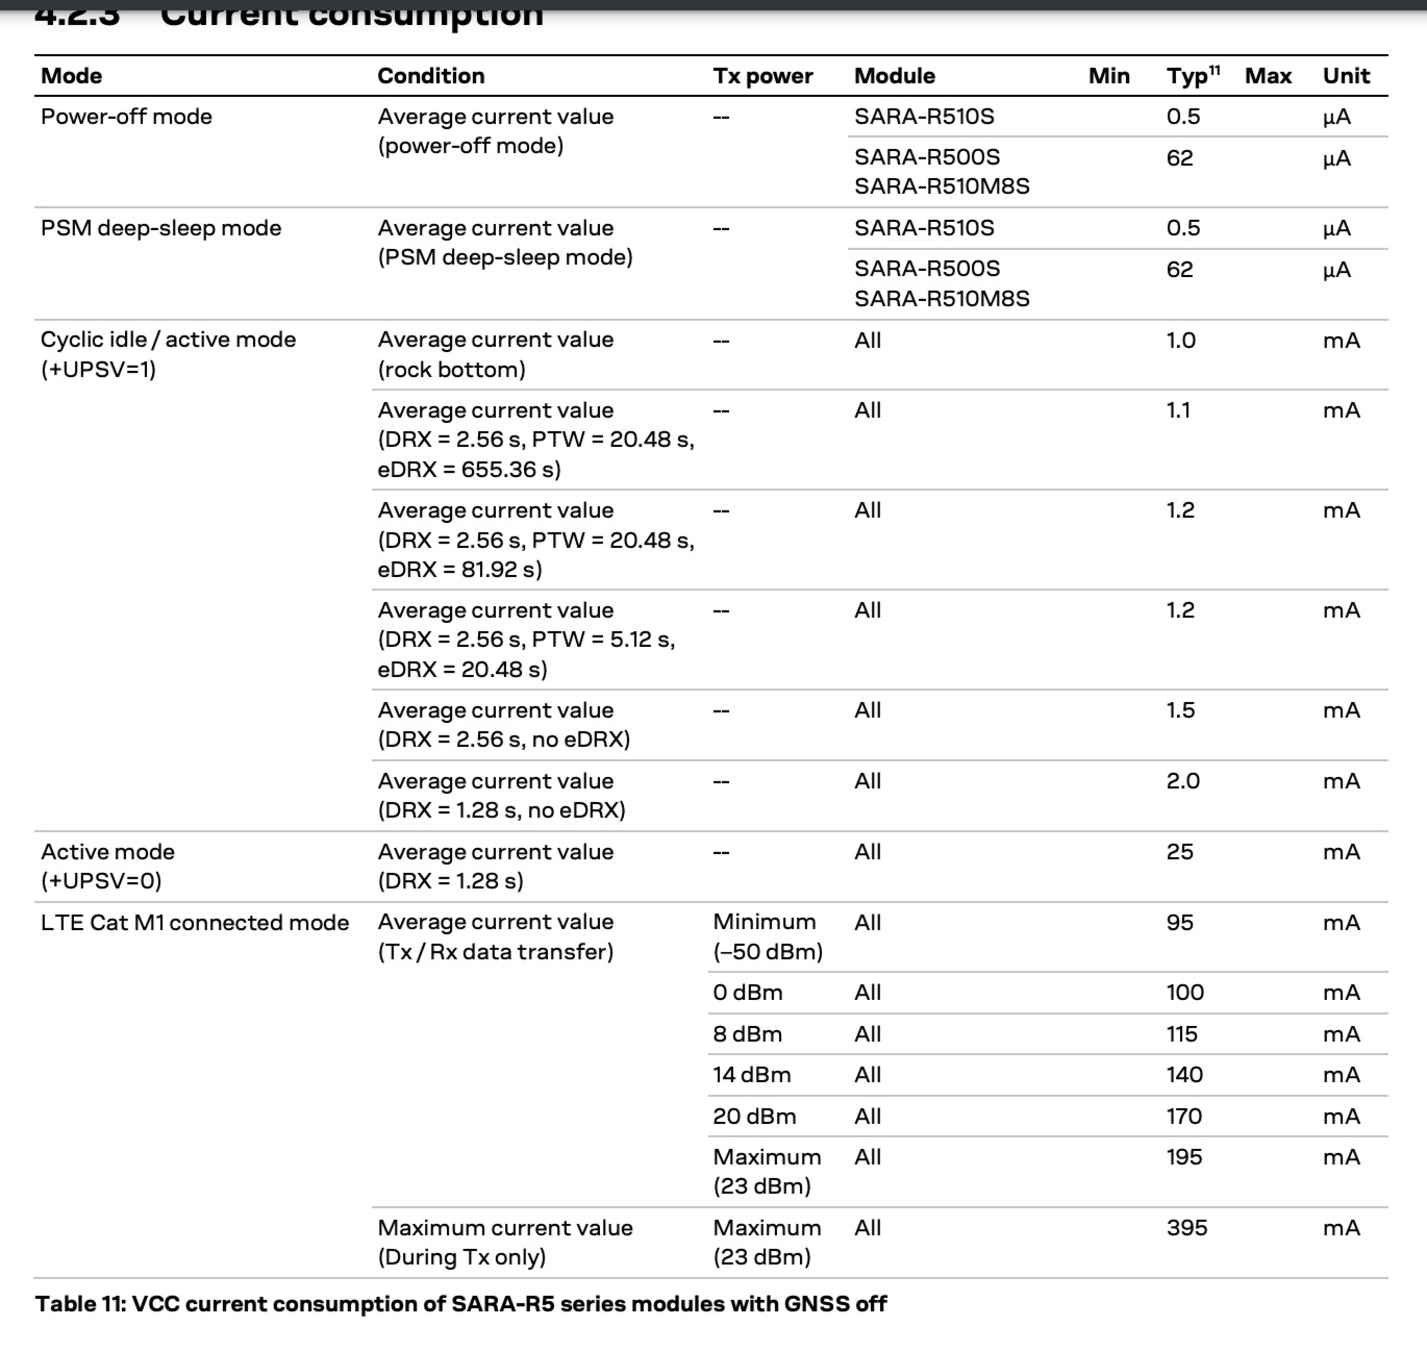
\includegraphics[width=\textwidth]{figures/NBTable.pdf}
    \caption{SARA Narrow-band IoT Module Power Consumption}
    \label{fig:NbTable}
\end{figure*}




%%%%%%%%%%%%%%%%%%%%%%%%%%%%%%%%%%%%%%%%%%%%%%

\bibliographystyle{ACM-Reference-Format}
\bibliography{refs}

\end{document}